\subsection{Component view}
In this section, components are expanded and better analyzed. \\
The main analysis regards the microservices block: 
\begin{figure}[H]
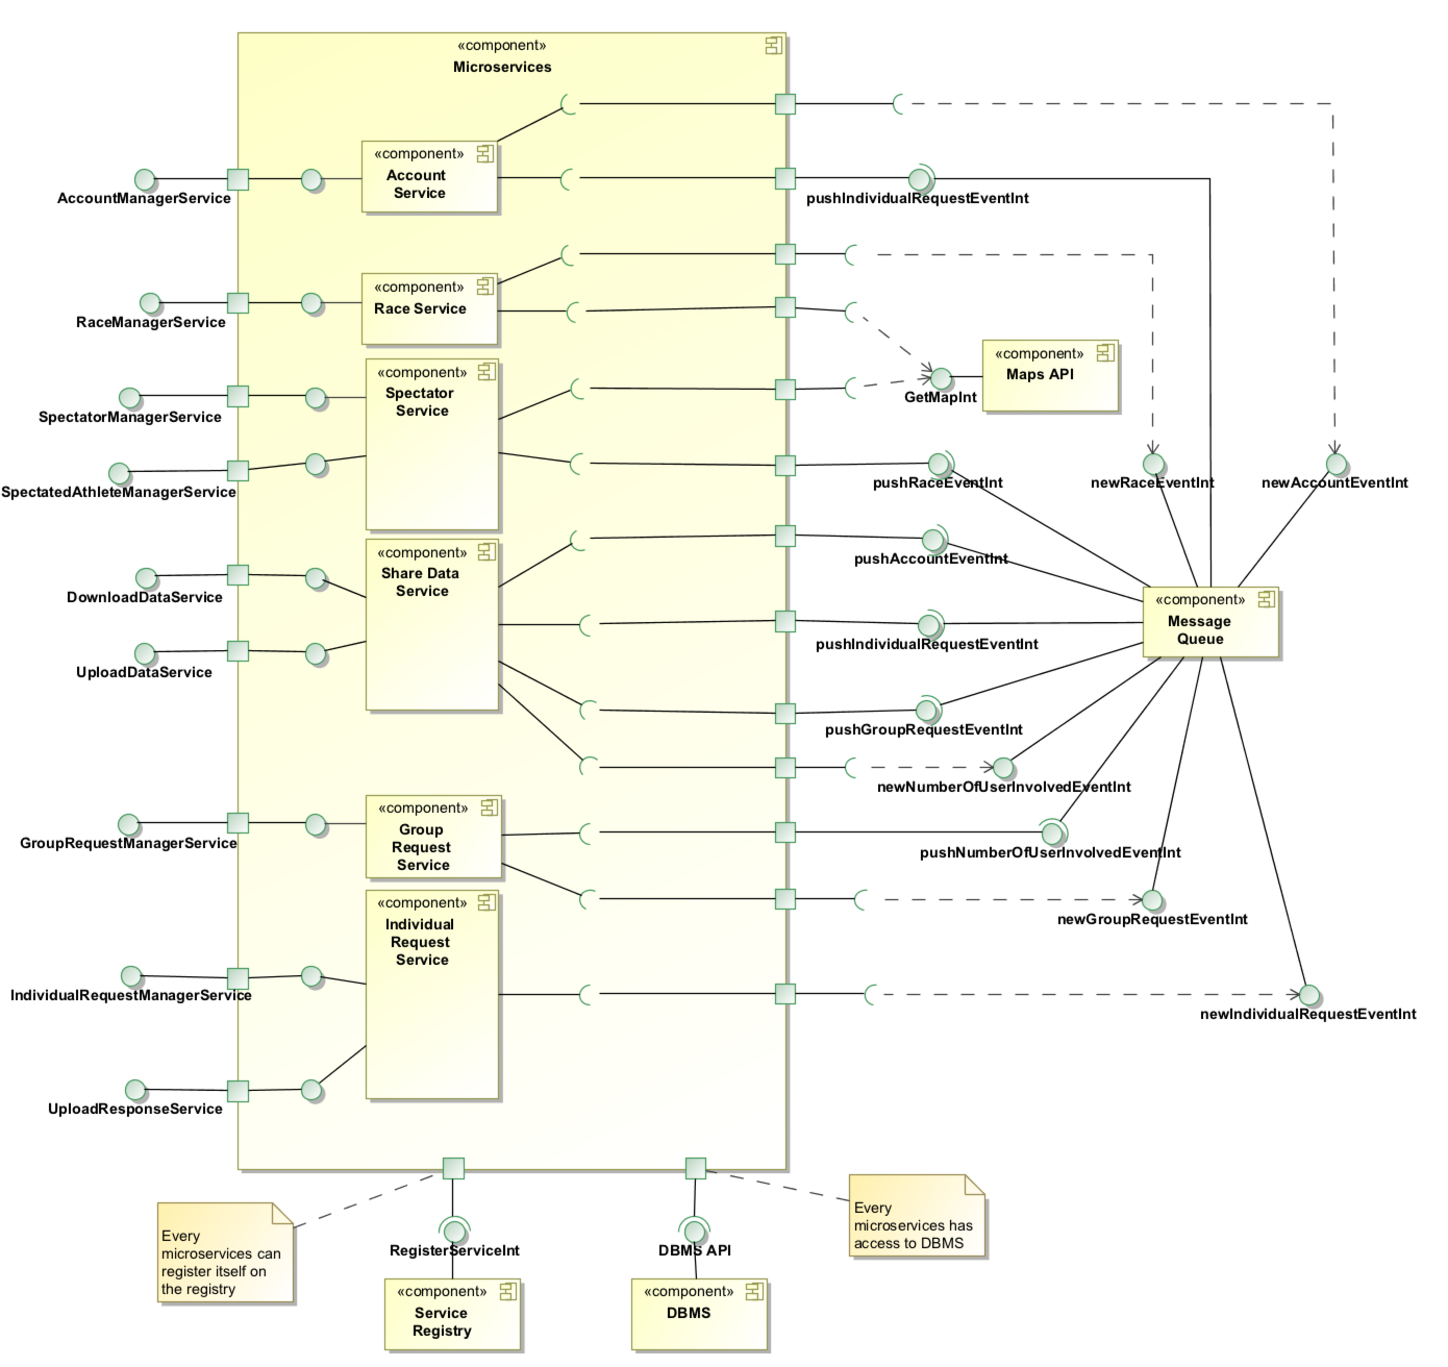
\includegraphics[width=\linewidth]{Images/componentdiagram.pdf}
\caption{ Component diagram }
\label{fig:componentdiagram}
\end{figure}
Various service components are present, and they all expose at least an interface that is accessed by the
clients via the API gateway. It follows a brief description of the various services, and a better
specification of the interfaces they provide to the API gateway:
\begin{itemize}
\item The account service provides all the functions related to user sessions, such as login and logout,
and also the registration of clients (both user and third party customer)
\item The race service makes possible for an athlete to enroll in a run; for a third party customer to set
up one, and also close it; and it also enables the possibility of retrieving the available races and their
status (e.g. in course, terminated). Therefore, it manages the "more static" part
of a race
\item The spectator service regards the dynamic part of a race, such as the fact that a user can spectate
the athletes who are running (therefore they can retrieve their positions and the leaderboard). This
service is also in charge of receiving position data of the participants
\item Share data service is responsible for the monitoring of user health statuses and positions: here a
user will upload his data. Furthermore, third party customer will access the data that they have
previously requested, by means of "DownloadDataService" interface
\item The group request service provides to the third parties the possibility of uploading group requests and see their status 
\item The individual request service enables third party customer to upload individual request and monitor their status, and allows a user to
check if there are some requests for him and upload responses 
\end{itemize}

Microservices have their own data and, therefore, access DBMS's API, while Maps's API are necessary 
only for race and spectator service, in order to manage and double check position data and feasible paths
\\
The diagram also shows the main communications that take place between components. The following message exchange is needed to completely and
correctly exploit the project functions. 
More specifically, when a third party is accessing individual data through the data share service, it
needs to know if a request associated with those data was sent and accepted. 
Indeed, the request acceptance and its data, are managed in the following way: the share data service provides an  interface that enables the
individual request service to communicate this event. \\ 
A slightly different reasoning holds for the management of the group requests. In this case, the exchange is bidirectional, and happens via
two different interfaces. 
In particular, when a new group request is performed, the share data service will be notified by the group request service, and it will check
the number of involved user.
After that, the share data service will communicate the response to the group request service: in this case it may happen that he status of
the request changes again, and, therefore, will be notified to the share data service again. Anyway, this will be later exposed and commented
in the run time view.  \\
The other important message exchange is between spectator and race services: in particular, data that the spectator service is receiving must
be matched with an active run, and thus it needs to know the status of the run: the change will be communicated by the interface exposed
by the spectator service. \\
It is possible to develop all the messages exchanged in an asynchronous way: this will prevent a possible slowdown of the application 
due to chains of synchronous calls.